\documentclass{article}
\usepackage{arxiv}
\usepackage[utf8]{inputenc} 
\usepackage[T1]{fontenc}    
\usepackage{hyperref}      
\usepackage{url}            
\usepackage{booktabs}       
\usepackage{amsfonts}       
\usepackage{nicefrac}       
\usepackage{microtype}      
\usepackage{cleveref}       
\usepackage{graphicx}
\usepackage{natbib}
\usepackage{doi}
%\usepackage{caption}
\usepackage{braket}
\usepackage{amsmath}
\usepackage{algpseudocode}
\usepackage{algorithm}
\usepackage{mathtools}
\usepackage{titlesec}
\usepackage[rightcaption]{sidecap}
\usepackage{wrapfig}
\usepackage{subfig}


\captionsetup[table]{skip=5pt}

\DeclarePairedDelimiter\floor{\lfloor}{\rfloor}

\setcounter{secnumdepth}{5}
\setcounter{tocdepth}{5}

\makeatletter
\renewcommand\subsubsubsection{\@startsection{paragraph}{4}{\z@}{-2.5ex\@plus -1ex \@minus -.25ex}{1.25ex \@plus .25ex}{\normalfont\normalsize\bfseries}}
\newcommand\subsubsubsubsection{\@startsection{subparagraph}{5}{\z@}{-2.5ex\@plus -1ex \@minus -.25ex}{1.25ex \@plus .25ex}{\normalfont\normalsize\bfseries}}
\makeatother

\title{Quantum Oracles - How to Transform Classical Problems into Quantum ones}

\date{\today}

\author{ 
	\href{https://orcid.org/0009-0008-9134-5974}{\includegraphics[scale=0.06]{orcid.pdf}\hspace{1mm}Alexandre Silva}\\
	Computer Science\\
	UNIVEM - Centro Universitário Eurípides de Marília\\
	\And
	\href{http://lattes.cnpq.br/5170103189904688}{\hspace{1mm}Luis Hilário Tobler Garcia} \\
	Computer Science\\
	UNIVEM - Centro Universitário Eurípides de Marília\\
	\And
	\href{http://lattes.cnpq.br/7265559606596355}{\hspace{1mm}Maúricio Duarte} \\
	Information Technology \\
	Fatec Garça – Deputado Julio Julinho Marcondes de Moura\\
}

\graphicspath{ {../images/} }

\renewcommand{\headeright}{}
\renewcommand{\undertitle}{}
\renewcommand{\shorttitle}{}


\hypersetup{
	pdftitle={Quantum Oracles - Como transformar problemas classicos em quanticos},
	pdfsubject={quantum computing, computer science, ciências da computação, computação quântica, algoritmos, algorithms, problem solving, problems, solução de problemas, problemas},
	pdfauthor={Alexandre Silva},
	pdfkeywords={quantum oracles, quantum, quantum computing, algoritmos, algorithms, problems, problemas},
}

\begin{document}

\maketitle

\begin{abstract}
	Using quantum oracles and other effects, like superposition, \emph{5 mini-projects} were done. The main goal of these projects was to answer if it's possible to bring some problems to the quantum realm and if such translation worth it. After finishing the tests, it was possible to see that, some of the implementations show descent results. However, classical computing is still a fundamental part of quantum algorithms.
\end{abstract}


\section{Introduction}
Now days, isn't difficult to hear someone talking about quantum computers, and how these machines will change the world. Nonetheless, the major fraction of these comments come from extrapolations and science fiction present in popular movies and series around the world. In this paper, I'm going to show that quantum computing it's not a magical trick to solve everything, but a tool for solving a distinct group of problems.\\
To do that, \emph{5 mini-projects} were implemented using \href{https://www.ibm.com/quantum/qiskit}{qiskit}, an open source framework from \href{https://www.ibm.com/}{IBM}, exploiting quantum effects and using classical/quantum algorithms to reach the expected outcomes. After that, the results will be here compared with their classical counterparts.
Such mini-projects are the following: Quantum File explorer\ref{file-explorer}, miles to kilometers conversion\ref{conversion}, Hanoi towers\ref{hanoi}, Buckshot Roulette \ref{buckshot} and QRAM \ref{qram}. All these implementations can be found at \href{https://github.com/Dpbm/scientific-initiation-1-quantum-oracles}{my GitHub repository}.

\section{Oracles}
Based on the idea of \emph{Oracle Turing Machines} \cite{SOARE2009368}\cite{amreen_oracle}\cite{kalyanasyndaram_2021_mod04lec23}\cite{e21080800}, the Oracles are mathematical modeling tools, used to abstract outlying parts of an algorithms into a black-box, making the algorithm analysis much easier. These machines could also be seen as a function, getting an input $x$ e returning $f(x)$ with time-complexity $O(1)$. Because of these unreachable characteristics for real life, this model can't be implemented, being used only for formal description of decision problems.\\
However, in quantum computing, it's possible to implement something similar to that, taking advantage of your inner structure and quantum effects to gain a \emph{Speed-up} relative to its classical counterparts, such Speed-up can be seen, for example, in the Deutsch–Jozsa algorithm \cite{Fan_2007}. Furthermore, the Quantum Oracles have a fundamental role determining the circuit complexity. Some approaches for that are: \emph{depth}, calculating the longest path in the circuit that some information must pass through and \emph{gate counting}, summing up how many gates were applied in the final circuit. Nevertheless, these approaches are very dependent of the \emph{QPU} topology, differing from each \emph{backend} used during the \emph{transpilation} process. To solve this problem, a well-known technique is to pack some parts of the circuit into Oracles, and then describing the complexity based on how many times they are called, it's also known as \emph{query complexity} \cite{odonnell_2015_lecture} \cite{e21080800}.

\subsection{Types of Oracles}
Using the base description of Quantum Oracles, we can classify them based on their structures and how the data is processed.

\subsubsection{Phase Oracle}
The Phase Oracle, is the most well-known format. Some Algorithms, like Deutsch–Jozsa, Grover, Simon and Bernstein–Vazirani, use it to take advantage over Classical approaches.

\subsubsubsection{Default Behavior}
As its main characteristic, the Phase Oracle adds a global phase to the circuit, using quantum effects like \emph{Phase Kickback} (basically the phase pass all the way through CNOT's target and is applied in the control Qubit), to change values in superposition.

\begin{figure}[h]
	\centering
	\includegraphics[scale=0.3]{phase_oracle_1.png}
	\caption{Phase Oracle using Phase-Kickback Example}
	\label{fig:phase-oracle-1}
\end{figure}

In the Figure \ref{fig:phase-oracle-1}, a $\pi$ phase was added in the auxiliary Qubit ($q3$), taking advantage of the phase $\ket{-}$, which will be the responsible to modify the values in the unitary matrix. In this setup, the $CNOT$ gates act slightly different from its default behavior, this way, the gate invert the value of the target Qubit and, due the $\pi$ phase, it also acts like a $Z$ gate applied in the control Qubit. So, after applying $CNOT\ket{-}\ket{+}$ (little-endian), the state becomes ${\frac{1}{\sqrt{2}}}{(\ket{0}\ket{-} - \ket{1}\ket{-})}$, and after removing the superposition, the final state is: ${\frac{1}{\sqrt{2}}}{(\ket{+}\ket{1} - \ket{-}\ket{1})}$. This way, the control Qubit is changed due the \emph{Phase Kickback} and its state is flipped from $\ket{0}$ to $\ket{1}$. Taking this effect as and advantage, we can use it to encode some binary values inside these oracles and use them to do some calculations.

\subsubsubsection{Minimal Oracle Version}

Furthermore, There's another layout possible for implementing a Phase Oracle. Once this one only applies a phase in some bit-strings, the auxiliary Qubit can be removed, and the phase can be provided by $CZ$ gates (or any other gate which can apply a phase for certain bit-strings). Doing that, it's possible to create a phase oracle keep its unitary and reversible nature, in the format of a minimal Oracle.

\newpage

\begin{figure}
	\centering
	\subfloat[\centering Phase Oracle - Minimal Oracle Layout Example]{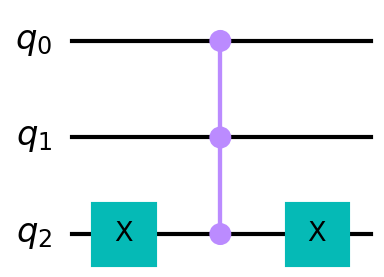
\includegraphics[width=5cm]{phase_oracle_2.png} \label{fig:phase-oracle-2}}
	\subfloat[\centering Figure \ref{fig:phase-oracle-2} Resulting Unitary Matrix]{\includegraphics[width=5cm]{phase_oracle_unitary.png} \label{fig:phase-oracle-unitary}}
	\caption{Phase Oracle Minimal Version}
	\label{fig:phase-oracle-minimal}
\end{figure}

In the example above \ref{fig:phase-oracle-minimal}, a $MCP$ gate was applied adding a $\pi$ phase and another two $X$ gates were used to invert the Qubits we want to have the value $0$ as a trigger for the $MCP$ phase application. Following the little-endian format the final encoded bit-string is: $011_{2}$ or $3_{10}$.

Looking at its unitary matrix \ref{fig:phase-oracle-unitary}, it's possible to see the $8\times8$ identity matrix with a $-1$ value in the column relative to the bit-string $011_{2}$, representing the encoded value.

\subsubsection{Boolean Oracle}

The Boolean Oracle has a similar structure with the Phase Oracle. However, this time a phase isn't applied, acting this way a regular boolean function, mapping inputs to outputs.

\begin{figure}[h]
	\centering
	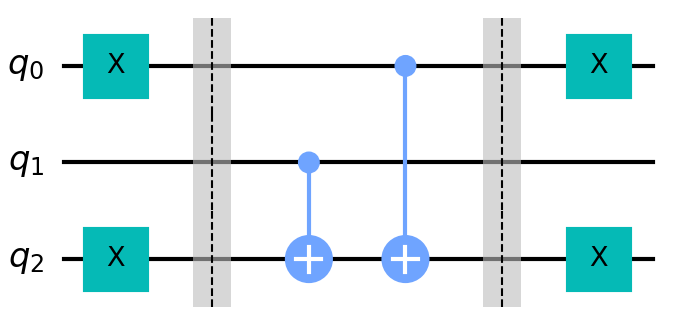
\includegraphics[scale=0.3]{balanced-oracle.png}
	\caption{Boolean Oracle Example}
	\label{fig:boolean-oracle}
\end{figure}

The example in the Figure \ref{fig:boolean-oracle}, is a well-known balanced Oracle for the Deutsch-Jozsa's algorithm. Nevertheless, to implement it, the Oracle must be transformed into a Phase Oracle.

\subsubsection{Minimal Oracle}
As previously mentioned, the Minimal Oracle is a function which its essence is unitary and reversible, so no additional Qubits are required. Therefore, this format can be either Boolean or Phase Oracle, depending on its implementation.

\newpage

\begin{figure}[h]
	\centering
	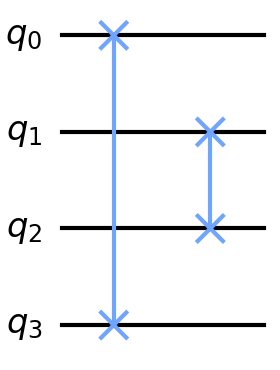
\includegraphics[scale=0.3]{minimal-oracle.png}
	\caption{Boolean Minimal Oracle example}
	\label{fig:minimal-oracle}
\end{figure}

The example \ref{fig:minimal-oracle} shows an Boolean Oracle which two $SWAP$ gates were used to invert the Qubits values order. Doing this way, the final matrix keeps its unitary and reversible properties, once the  $SWAP$ gates act in both Qubits together, mirroring its action.


\subsubsection{QFT(Quantum Fourier Transform)}
The QFT is, in a nutshell, a quantum algorithm based on the Discrete Fourier Transform, used for quantum states period finding, projecting values from the computational basis onto the $X$ basis (also know as Fourier basis).

Even though it's an algorithm by itself, its application is done in the format of Oracles in quantum circuits.


\begin{figure}[h]
	\centering
	\subfloat[\centering QFT Oracle example]{\includegraphics[scale=0.3]{QFT_1.png} \label{fig:QFT}}
	\subfloat[\centering Values Mapped onto Fourier basis example (quantum state $\ket{000}$)]{\includegraphics[scale=0.2]{QFT_1_bloch.png} \label{fig:QFT-bloch}}
	\caption{QFT Oracle}
	\label{fig:QFT-oracle}
\end{figure}


\subsubsection{Other kinds of Oracles}
In addition to the oracles mentioned above, it's possible come across with different mentions of Oracles, like the Simons's, Deutsch-Jozsa's, etc. However, these are just implementations of models already shown in this paper. Also, the most relevant for the following projects are the Phase and Boolean ones, due that, there's no use to keep discussing about many others sub-categories of Oracles here.

\section{Development}


\subsection{File Explorer} \label{file-explorer}
Imagine a quantum computer, but instead of one of those we already have in real life, imagine a different kind, very similar to those we have at home, with a quantum operational system, quantum files, etc. This imaginary version could be thought as a hybrid computer as well, taking advantage of both quantum and classical capabilities. Using this idea, the first project implements a file explorer for this ideal system.

\newpage

\subsubsection{Algorithms Used}

\subsubsubsection{Grover}
The Standard algorithm for search problems is the Grover's algorithm. This one, realizes searches on unsorted "databases" (bit-string in this case) with $O(\sqrt{2^n})$, being $n$ the number of Qubits. Its tenets are based on amplitude amplification, using a Phase Oracle to mark some bit-strings and then using a Diffuser to amplify the probability to find these values after measuring it.

\begin{figure}[h]
	\centering
	\includegraphics[scale=0.25]{Grover.png}
	\caption{Example Grover's algorithm with $3$ Qubits}
	\label{fig:grover-default-circuit}
\end{figure}

For building the circuit, is needed a joint of $Oracle + Diffuser$ applied $k$ time, which $k \approx { {\frac{\pi}{4 \sqrt{\frac{a}{2^n}}}} - {\frac{1}{2}}  }$, being $a$ the number of values marked by the Oracle. Once we want to find just a single file, the use of this relation is not required, being need to apply the algorithm once to find the bit-string.

Even this being the best option for bit-string finding, in this project different rotations were tested trying to find a better superposition which increases the chances to find the value we want.

\begin{SCfigure}[0.6][h]
	\caption{Comparing the Standard Grover's algorithm with the version modifying the rotation angles $[0, 2\pi]$ for each 4 bits bit-string}
	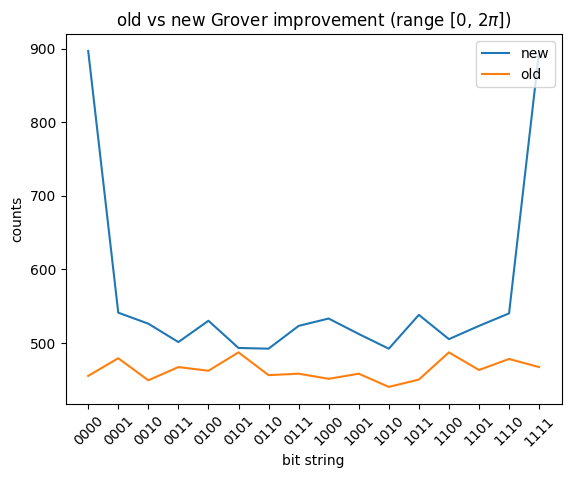
\includegraphics[width=8cm]{improvement-grover-algorithm-4bits-0-to-2pi.png}
	\label{fig:best-angle-grover}
\end{SCfigure}

\newpage

Using specific rotations for each bit-string, it's possible to improve the outcomes, and even stand out the default rotation.

\begin{figure}[h]
	\centering
	\includegraphics[scale=0.4]{new-grover-test-different-bit-strings-with-optimal-angles.png}
	\caption{Test Using the best angles of each bit-string in different ones}
	\label{fig:best-angles-diff-bit-strings-grover}
\end{figure}

However, using the best angle of a distinct bit-string as the source of superposition in the algorithm, isn't enough to overcome the classical Grover implementation, and also the probability distribution becomes irregular. So, for a general purpose implementation, the default rotation is the best one for the most part of the cases. This behavior is even weird with $2$ Qubits, being the $H$ gate rotation the best ever for that.


\begin{figure}[h]
	\centering
	\subfloat[\centering Results for Grover with 2 Qubits (default rotation)]{\includegraphics[scale=0.3]{classical_grover_for_1_bit_strings_l2_outcomes.png} \label{fig:l2-grover-classical-outcomes}}
	\subfloat[\centering Results for Grover with 2 Qubits (modified rotation)]{\includegraphics[scale=0.3]{new_grover_for_1_bit_strings_l2_outcomes.png} \label{fig:l2-grover-new-outcomes}}
	\caption{Comparing Grover with 2 qubits using the default and modified rotation}
	\label{fig:comparing-grover-2-qubits}
\end{figure}

For our purpose in this project, the hybrid approach was used. So during the circuit setup, the searched value pass through a Hash-Table will optimal angles. This way, the algorithm can achieve better outcomes at the end of the execution, finding, this way, the file we want. 

\subsubsubsection{Sets Difference}
Overlapping two distinct Phase Oracles, each one with a range of values encoded. The remaining Phases, are the difference of the sets encoded by them \cite{sanchezrivero2023initial}.

\newpage

\begin{figure}[h]
	\centering
	\subfloat[\centering Sets Difference Algorithm Example]{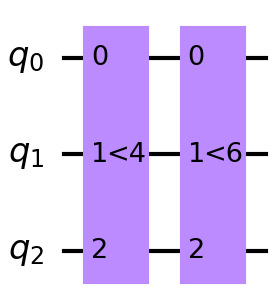
\includegraphics[scale=0.4]{less_than.png} \label{fig:less-than-circuit}}
	\subfloat[\centering Unitary After applying the Sets Difference algorithm]{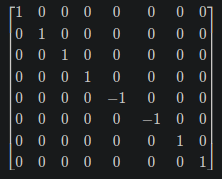
\includegraphics[scale=0.5]{less_than_unitary.png} \label{fig:less-than-circuit-unitary}}
	\caption{Sets Difference example}
	\label{fig:sets-diff-example}
\end{figure}


In the last example \ref{fig:less-than-circuit}, the set $\{000, 001, 010, 0110\}$ was encoded in the first Oracle and $\{000, 001, 010, 011, 100, 101\}$ in the second one.

After Overlapping the phases  \ref{fig:less-than-circuit-unitary}, only the values $\{100, 101\}$ keep the $-1$ value. This way, we can do the set operation just applying some oracles with the values range we want.

\subsubsection{Final Solution}


As a solution for this problem, a hash function was made, mapping the path of some file $p$ to a specific bit-string $b$, $F: p \to b$. With this function, we can use a set returned values and encode them into a Phase Oracle, creating a sort of quantum Look-Up-Table for files in that machine. Moreover, a second Oracle containing all the bit-strings, with the exception of the searched one, is applied for difference of sets algorithm, this way the phases will be overlapped, and only the one we want will pass to the Grover's algorithm.


\begin{figure}[h]
	\centering
	\includegraphics[scale=0.4]{sets-difference-look-up-table-oracle.png}
	\caption{Look-up-Tables applied}
	\label{fig:luts}
\end{figure}


Finally, the modified version of the Grover's algorithm is applied.

\begin{figure}[h]
	\centering
	\includegraphics[scale=0.4]{improved_file_explorer.png}
	\caption{File explorer final circuit}
	\label{fig:file-explorer}
\end{figure}

This setup, maximizes the probability to find the queried file, presenting the following distribution after $1000$ shots.

\begin{figure}[h]
	\centering
	\includegraphics[scale=0.6]{AER-file-explorer-hist-new-grover-mapped-rotations.png}
	\caption{ File Explorer Results after running with Qiskit-AER}
	\label{fig:file-explorer-hist}
\end{figure}


\subsubsection{Results}

For this specific ideal case, it is, probably, one of the best known ways to do the search between "quantum files".

However, it's not the best alternative as a way to speed-up classical searches. It happens because storing a large Look-Up-Table for encoded files and another one for keeping track of each optimal angle for every bit-string contained between $2^n$ combinations, could be really costly and slow. Also, it would be required a hash function with a tiny probability of collision.

An alternative for that could be using the standard Grover's algorithm, but it still the need to encode the hard drive files to a big table. Also, comparing the classical tree approach with Grover's, their worst cases scenarios are $O(log(n))$ and $O(\sqrt{n})$, which implies that the first one still faster than the later. As a last point, the quantum version for this problem, could present the wrong file after searching due errors and the quantum randomness.

Keeping that in mind, the final algorithm is a right choice for a quantum system as describe at the beginning of this section, but it can't overcome the best algorithm in a classical computer. 



\subsection{Miles to Kilometers Conversion} \label{conversion}

The second problem that was tested here, was the conversion from miles to kilometers. This idea came out after finding a quantum algorithm capable of calculate the Fibonacci sequence, which is an essential piece for this very project.
 
\subsubsection{Used Algorithms}

\subsubsubsection{Quantum Fibonacci}

The quantum version of Fibonacci was presented in \cite{gilliam2020canonical}. This paper shows that, using a quantum circuit with all bit-string in superposition, and then apply  controlled rotations to remove values that contains consecutive ones, is possible to approximate the result of the \textit{n}-th Fibonacci sequence value.

\newpage


\begin{figure}
	\centering
	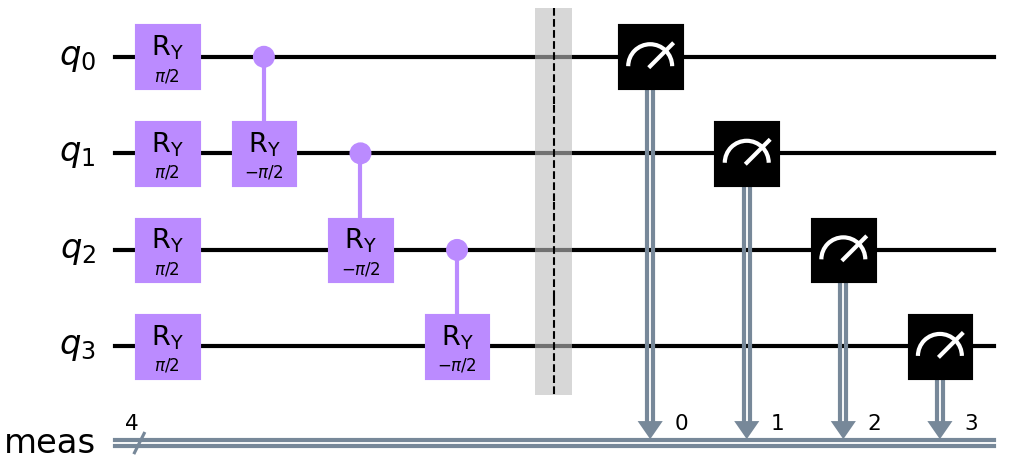
\includegraphics[scale=0.3]{fibonacci-circuit.png}
	\caption{Quantum Fibonacci Example}
	\label{fig:fibonacci-circuit}
\end{figure}

\begin{figure}
	\centering
	\includegraphics[scale=0.4]{fibonacci-4.png}
	\caption{Quantum Fibonacci result - F(4)}
	\label{fig:fibonacci-circuit-result}
\end{figure}

After running the circuit $k$ times, the amount of unique bit-string that appeared during the experiment represent the \textit{n}-th Fibonacci value, which $n$ is the total of Qubits were used in the circuit. So, for the example \ref{fig:fibonacci-circuit} above, the position $n$ we want, is $4$, and the result after counting the bars of which values are $\neq 0$ give us the result of $F(4) = 8$.

It may seem wrong, however, the quantum setup differ slightly from the classical one, once the first value is $2$ instead of $1$, this way, the sequence is: $F(1)=2, F(2)=3, F(3)=5, F(4)=8, F(5)=13, F(6)=21, ...$, which implies that it worked for this example.


\subsubsubsection{Approximating Miles to Kilometers}

To approximate the value from miles to kilometers, an old approach for that is using the Fibonacci sequence. This method, uses the relation $F_{km} = F_{milhas}(n+1)$, which $F$ is the classical Fibonacci algorithm ($F(1) = 1$ and $F(2) = 2$), and $n$ is a known position in this very sequence. Following this equation, the relative kilometers values will be given in the next \textit{n} ($n+1$). 

\begin{table}[h]
	\begin{center}
		\begin{tabular}{ |c|c|c| } 
			\hline
			miles & Km & Real(Km) value\\
			\hline
			1 & 2 & 1.60934\\
			\hline
			2 & 3 & 3.21869\\
			\hline
			3 & 5 & 4.82803\\
			\hline
			5 & 8 & 8.04672\\
			\hline
		\end{tabular}
	\caption{Approximated miles-Km values}
	\end{center}
\end{table}

\newpage

For values that aren't present in the sequence, they can be generated combining multiple values which are there. For example, to transform $10$ miles to kilometers, we could use the values $8$ and $2$, which are known in the sequence, and then used the previous cited method for each part. So, for this example, $8 = F(5)$ and $2 = F(2)$, so $F(5 + 1) + F(2 + 1) = F(6) + F(3) = 13 + 3 = 16Km$ giving a close value of $\approx 16.0934Km$.


\subsubsection{Implementation}

Using the formulation above, the final algorithm takes place using a Hybrid approach, following the structure bellow:

\begin{algorithm}[h]
	\begin{algorithmic}
		\State{parts = $BreakInputIntoFibonacciParts(input)$}
		\For{parte in parts}
			\State{Apply the Oracle embedding $F(part)$}
			\State{Measure the Oracle Qubits}
			\State{Reset these Qubits}
		\EndFor
		\State{Check the outcomes}
		\State{Multiply the given result for its relative $i$}
			
	\end{algorithmic}
	\caption{Quantum Conversion algorithm}
	\label{alg:miles-to-km-quantum-algortihm}
\end{algorithm}

In this algorithm, is needed a preprocessing routine, using a classical algorithm, to split the input number into smaller parts that can be calculated using the sequence. Also, to reduce the amount of Oracle applications to decrease the quantum noise, this processing returns a tuple for each number containing $n$ and the total of applications needed $p$, this way, we can apply each Oracle once and after retrieving the outcomes, the final result is giving by: $\sum_{i=0}^{m} {o_{i}p_{i}}$, being $m$ the total of parts and $o$ the given output.


% fix this one (put each relative number in the Oracle name)
\begin{figure}[h]
	\centering
	\includegraphics[scale=0.18]{number_breakdown_circuit.png}
	\caption{Final Miles to Kilometers Circuit}
	\label{fig:miles-km-circuit}
\end{figure}


\subsubsection{Thoughts on the Results}

With this method, is possible to evaluate some input values. However, there are some points which make it unfeasible.

\begin{description}

\item[Execution Time]{Each part to be calculated, takes too much \emph{shots}, taking around $500-10000$ to get better results, therefore increasing the execution time}

\item[Errors]{Due the high depth of this kind of circuit, this setup is likely to present wrong results due multi-Qubit operations in real hardware}

\item[Impression]{After running the algorithm for many different values, it's clear that, for large numbers, the output deviates a lot from what the expected was}

\item[Classical Intervention]{Once it requires both pre and post-processing using classical algorithms, the usefulness of the quantum version decreases}
\end{description}

\newpage

\begin{figure}[h]
	\centering
	\includegraphics[scale=0.35]{miles_to_km_defiance.png}
	\caption{Comparing the precision between classical and quantum versions}
	\label{fig:values-miles-km-quantum}
\end{figure}

Thus, this protocol can be used for small numbers. However, to be useful as its classical version, it should be more resilient to errors and precision issues, also it needs to be more independent from classical computations, once most of the work is based on classical routines.

Consequently, this final algorithm isn't good as the classical one, and probably isn't useful enough for real applications. Nonetheless, it's possibly a starting point for different approaches for real implementations. 

\subsection{Hanoi Towers} \label{hanoi}

For the Hanoi Towers implementation, it was designed a way to encode the discs positions in the tower using their binary values and the Phase Oracle as a storage device.

\subsubsection{Implementation}
This project, requires $(\floor{\log_2{x}} + 1) * 3$ Qubits, being $x$ the number of disks. The Qubits layout follows this sequence: $\ket{t_{n-1} t_{n-2} ... t_0}\ket{a_{n-1} a_{n-2} ... a_0}\ket{s_{n-1} s_{n-2} ... s_0}$, where $s$,$a$,$t$ are the first, second and third towers respectively.

To prepare the state, a Phase Oracle is prepared encoding each disc number (from $1$ to $x$) in the first rod (Qubits $s$) using the global phase $\pi$. After that, $SWAP$ operations are done following the classically preprocessed steps, moving bit-by-bit from one rod to another.

\newpage

\begin{figure}[h]
	\centering
	\includegraphics[scale=0.3]{hanoi_3_discs.png}
	\caption{Quantum Hanoi Tower with 3 disks}
	\label{fig:hanoi}
\end{figure}

As cited previously, the movements are preprocessed before playing. This way,the quantum setup acts like a classical player, executing step-by-step his strategy.

Also, as we're playing with phases, it's possible to apply phase amplification algorithm, like Grover's, to evaluate the tower and get the resulting values.

\begin{figure}[h]
	\centering
	\includegraphics[scale=0.5]{result_hanoi_3_discs.png}
	\caption{Quantum Hanoi Tower with 3 disks - evaluation using Grover's algorithm}
	\label{fig:hanoi-result}
\end{figure}

As shown in \ref{fig:hanoi-result}, after evaluating the circuit, it's possible to see $3$ high probability bit-strings, which represent the encoded disks. These bit-string are $010000$, $100000$ and $110000$, so the operations moved successfully the disks from the source rod (rightmost $2$ bits) to the target rod (leftmost $2$ bits).

\subsubsection{Thoughts on the Results}

Once it followed the same sequence of implementation as the classical one, requiring, inclusively, preprocessing. This version is equivalent to the classical algorithm, keeping in mind that for a classical computer, it's also required to precompute a movement, and then play it.

\newpage

\subsection{Buckshot Roulette} \label{buckshot}
\emph{Buckshot Roulette} is a computer game made by \href{https://mikeklubnika.itch.io/}{Mike Klubnika}, based on the idea of modifying the infamous Russian Roulette. 

During the game, you are challenged to play against a demon (dealer). If you win, you'll receive a prize, otherwise the game will restart and you can try again.

In this very project, we analyzed the first game match, trying to find the best strategy to maximize the player's winnings. The reason for choosing the first match, is because of its simplicity, being away from power-ups that could complicate the analysis, and also because this one shows the base dynamics for the entire game, so doing well in this one, is the first step to beat the whole game.

\newpage

\subsubsection{Dinâmica}
Na rodada, são colocadas $2$ balas falsas e $1$ bala verdadeira na arma, sendo o player o primeiro a jogar. Ambos os jogadores podem escolher entre atirar em si mesmo, ou em seu oponente. Assim, a próxima ação é estritamente depende das probabilidades de ser uma bala real ou falsa. A partir dai, a dinâmica funciona da seguinte forma: 

\begin{algorithm}[H]
	\begin{algorithmic}
		\If{jogador escolhe atirar no dealer}
			\If{bala for real}
				\State{Jogador ganha a rodada}
			\Else
				\State{Dealer joga a próxima}
			\EndIf
		\Else
			\If{bala for real}
				\State{Jogador perde}
			\Else
				\State{Player joga a próxima}
			\EndIf
		\EndIf

	\end{algorithmic}
	\caption{Possíveis jogadas}
	\label{alg:buckshot-roulette}
\end{algorithm}

Essa dinâmica se repete a cada jogada, sendo válida tanto para o dealer, como para o player.


\subsubsection{Versão clássica}
Para entender melhor a dinâmica, é possível representar cada ação e suas consequências em formato de árvore. Dessa forma, cada jogada leva a partida para mais próximo do fim.


\begin{center}
	\includegraphics[scale=0.2]{buckshot-roulette-diagram.png}
	\captionof{figure}{Buckshot Roulette diagrama de árvore}
	\label{fig:classical-model-bckr}
\end{center}

Nessa estrutura, é previsto que o jogador seja um agente racional, e o dealer uma máquina com ações aleatórias. Assim, o jogador sempre visa o seu próprio benefício, enquanto o dealer age pela sorte.Tal comportamento pode ser visto nas folhas da árvore do qual, sempre que o player é o próximo jogador, sua ação é apenas atirar no adversário, enquanto o dealer ainda possui a possibilidade de entregar o jogo atirando em si próprio, mesmo havendo apenas uma bala na arma e, pela lógica do jogo, ser uma bala verdadeira.\\
Seguindo essa estrutura, podemos simular os possíveis caminhos e verificar a melhor estratégia.

\begin{center}
	\includegraphics[scale=0.6]{optimal_player_strategy.png}
	\captionof{figure}{Buckshot Roulette clássico - melhor estratégia}
	\label{fig:classical-model-bckr-optimal-strategy}
\end{center}

Após testar os caminhos possíveis, o melhor resultado obtido foi esse apresentado acima em \ref{fig:classical-model-bckr-optimal-strategy}. Com um pouco de investigação, foi possível entender que essa estratégia se baseia no jogador começar atirando no dealer. Isso acontece, pois, ao seguir tal caminho, ele tem uma chance a menos de perder a rodada ao atirar em si mesmo logo no começo da partida.

\begin{table}[!h]
	\begin{center}
		\begin{tabular}{ |c|c|c|c| } 
			\hline
			rodada & ação & resultado da ação & resultado da partida \\
			\hline
			1 & player atira no dealer  & real & player ganha\\
			\hline
			1 & player atira no dealer  & fake & -\\
			\hline
			2 & dealer atira no player  & real & dealer ganha\\
			\hline
			2 & dealer atira no player  & fake & -\\
			\hline
			2 & dealer atira nele mesmo  & real & player ganha\\
			\hline
			2 & dealer atira nele mesmo  & fake & -\\
			\hline
			3 & player atira no dealer  & real & player ganha\\
			\hline
			3 & dealer atira no player & real & dealer ganha\\
			\hline
			3 & dealer atira nele mesmo  & real & player ganha\\
			\hline
		\end{tabular}
		\caption{melhor estratégia - possíveis resultados}
	\end{center}
\end{table}

\subsubsection{Versão quântica}
Para a versão quântica, um circuito foi modelado imitando o funcionamento do game. Nesse algoritmo, um Oracle foi usado para cada jogador, implementando internamente sua estratégia.

\begin{center}
	\includegraphics[scale=0.3]{quantum_buckshot_roulette.png}
	\captionof{figure}{Circuito para o Buckshot Roulette}
	\label{fig:bckr-circuit}
\end{center}

Além disso, para encontrar a estratégia, foram inseridos dois parâmetros dentro do Oracle do player, sendo possível configurar qualquer valor $\theta$ e $\phi$ para modificar a rotação na Bloch Sphere.\\
Após verificar os possíveis valores, a rotação que entregou o melhor resultado foi $\theta\approx 3.0853981633974477, \phi\approx3.7853981633974474$ radianos. Usando essa estratégia, os resultados foram semelhantes a versão clássica.

\begin{center}
	\includegraphics[scale=0.6]{final_buckshot_roulette_quantum_optimal_strategy.png}
	\captionof{figure}{Resultado Buckshot Roulette quântico - Qiskit AER}
	\label{fig:bckr-circuit-result}
\end{center}

Observando a Bloch Sphere do estado gerado por essa rotação, é possível ver também que a estratégia se aproxima da versão clássica, com o player preferindo atirar no dealer a maior parte do tempo (o valor $1$ representa atirar no outro jogador e $0$ em si mesmo).

\begin{center}
	\includegraphics[scale=0.6]{player_optimal_strategy_bloch.png}
	\captionof{figure}{Melhor estratégia Buckshot Roulette quântico - Bloch Sphere}
	\label{fig:bckr-bloch-sphere-best-strategy}
\end{center}

Como uma última nota sobre o circuito, no exemplo \ref{fig:bckr-circuit-result}, o total de partidas ganhas por cada jogador não chega ao total jogado (nesse caso $1000$ partidas foram simuladas). Isso acontece devido ao design do circuito, o qual não é possível verificar a jogada do player anterior, acarretando na continuação do jogo mesmo que um dos players já tenha perdido, o que cria a necessidade do uso de pós processamento para limpar os resultados inválidos.

\subsubsection{Conclusões}
Para esse problema, não há uma competição certa entre as duas versões, já que uma é diretamente inspirada na outra. Contudo, a versão quântica possui ainda a possibilidade de explorar mais valores do que a versão clássica, deixando o player mais aberto a escolha de novas estratégias, o que pode ser visto como um ponto a favor da versão quântica.\\
Em suma, ambos as simulações atingiram o mesmo resultado e foi demonstrado que é possível usar o quantum Oracle como uma representação de um player dentro do circuito.

\subsection{QRAM} \label{qram}
Por fim, o último projeto realizado foi o de uma \emph{QRAM} utilizando os Oracles. Nessa versão, foi testado a criação de \emph{QROMs} (com dados estáticos dentro), e uma possível maneira de utilizar uma QRAM hábil para escrita.\\
Neste projeto, foi tido como objetivo o armazenamento de estados quânticos (superposições), e não apenas de bit-strings clássicas. Isso pois, para garantir a real eficiência da computação quântica, a superposição é indispensável, e seu armazenamento pode ser um ponto chave para algoritmos melhores.

\subsubsection{QROM}
Para a QROM, são utilizados $n$ qubits para o barramento de endereços e $m$ qubits para a o barramento de dados, sem a necessidade desses valores estarem correlacionados, podendo assim ser utilizado, por exemplo, $n=3; m=10$. Nessa estrutura, podemos mapear diversas superposições diferentes e aplicá-las quando certo endereço for chamado. Sendo assim, o algoritmo armazena os valores a partir da configuração de gates controlados interiores ao Oracle, criando uma superposição apenas quando certo valor de entrada é inserido, seguindo o formato: ${\ket{0}^{\otimes m}} {\ket{a_{n-1} a_{n-2} ... a_0}}$.

\begin{center}
	\includegraphics[scale=0.5]{qrom_1.png}
	\captionof{figure}{Exemplo circuito - QROM}
	\label{fig:qrom}
\end{center}


Em \ref{fig:qrom}, $q_{0}$ age como o barramento de endereços, enquanto $q_{1}$ como o barramento de dados. Aqui configuramos para mapear o endereço $0 \to RY({\pi\over{3}})$ e $1 \to H$. Sendo assim, para $n$ qubits no barramento de endereços é possível mapear para $2^{n}$ estados, e com os $m$ qubits é possível criar estados mais complexos aumentando sua quantidade e utilizando outros gates acionados para um mesmo endereço. \\
A partir da abstração desse circuito para um Oracle,é possível utilizar a QROM em um circuito maior, chamando-o novamente sempre que for necessário um certo estado. Além disso, no formato de Oracle, há a possibilidade de colocar os endereços em superposição e ter uma mistura de estados na saída.

\begin{center}
	\includegraphics[scale=0.5]{qrom_1_usage.png}
	\captionof{figure}{Exemplo circuito usando a QROM com endereços em superposição}
	\label{fig:qrom-usage}
\end{center}

Nesse exemplo \ref{fig:qrom-usage}, os endereços são colocados em superposição no qubit \emph{addr} e assim os estados em internos do Oracle são colocados em uma sobreposição de $50-50$ no qubit \emph{out}. Com isso, pode-se aproveitar do resultado de \emph{out} em outros qubits, como nesse caso o qubit \emph{q}.\\
Contudo, devido ao no-cloning-theorem, não é possível copiar esse estado para outro qubit alvo. Sendo assim, não é possível ter dois qubits com o mesmo estado a partir daquele armazenado, podemos apenas pegar o resultado de uma superposição e utilizar o valor binário como trigger para outra operação.\\
Uma opção para solucionar isso, é utilizar o teleporte quântico, destruindo assim o estado interno do Oracle e movendo-o para outro qubit desejado.

\subsubsection{QRAM}
Para criar uma QRAM com a possibilidade de escrita, o teleporte quântico, já citado anteriormente, é um caminho para isso. Com ele, podemos ter $n$ qubits, sendo cada qubit um endereço único, e utilizar do teleporte para mover um estado que estava no circuito, para o domínio da QRAM.

 \begin{center}
 	\includegraphics[scale=0.4]{qram.png}
 	\captionof{figure}{Exemplo circuito - QRAM}
 	\label{fig:qram}
 \end{center}

Aqui, os $n$ qubits agem tanto como endereços quanto dados (qubits \emph{data}). Além disso, são necessários mais $n$ qubits para o teleporte (qubits \emph{t}).\\
Com isso, é possível ver que o circuito cresce de forma linear a medida que mais endereços são requisitados, sendo assim $O(2*n)$ em relação à quantidade de qubits total.\\
Na configuração acima \ref{fig:qram}, é possível sobre-escrever valores, assim como interferir com outras superposições apenas teleportando novos valores para o qubit $i$. Dessa forma, podemos criar uma memória menor e, conforme necessário, remover e adicionar outros valores.

\subsubsection{Conclusões}
Com esse projeto, e com a literatura usada \cite{jaques2023qram}\cite{Giovannetti_2008}, é possível entender que criar versões quânticas de memória é uma tarefa desafiadora, e ainda não é possível tomar proveito de todo o seu potencial usando as superposições e estados de outras bases a não ser a base computacional $({0,1})$. Fatores como, complexidade de mapear dados, complexidade de utilizar a memória (já que é necessário reaplica-lá toda vez que for requisitado seu uso), no-cloning-theorem, decorrência, etc. Influenciam diretamente na possibilidade de sua criação.Mesmo sendo possível implementar pequenos circuitos que agem como memória, como os mostrados aqui, ainda não é usual e muito menos universal para qualquer tipo de máquina quântica.\\
Além disso, por esses fatores, a QRAM, pode dificultar a execução de múltiplas tarefas, uma vez que o valor presente nela não pode ser copiado, e ao move-lo para outro qubit, o valor anterior da QRAM é completamente destruído.\\
Como mostrado na literatura, para resolver esses problemas, o melhor approach para a sua implementação, é a utilização de um hardware especifico para essa finalidade, sem a intervenção de circuitos quânticos.\\ 
Em suma, mesmo sendo possível criar pequenos circuitos para implementar uma memória, seu uso está longe de se comparar as versões clássicas.

\subsection{Conclusão}
Perante o exposto, foi evidenciado que a computação quântica ainda tem muito potencial. No entanto, é possível ver que certos fatores, e a falta de alguns recursos, prejudicam o seu uso no momento.\\
Como já mostrado pelas inúmeras pesquisas em áreas como, química, machine learning, criptografia, otimização, etc. A computação quântica pode, num futuro próximo, ser um ponto crucial para conseguir resultados mais precisos e, em certos casos, em menor tempo.\\
No entanto, na era NISQ, para conseguir utilizar todo seu potencial, é necessário ter em conjunto máquinas clássicas para pré e/ou pós processamento, seja para executar alguma tarefa computacionalmente custosa para um computador quântico, ou para o uso de algoritmos de detecção e correção de erros. Como demonstrado aqui, ao utilizar esse conjunto, é possível ter o melhor dos dois mundos, mesmo que na maioria do casos, esse formato de implementação não se sobressaí as versões já utilizadas classicamente, com o tempo e o aperfeiçoamento das técnicas e do hardware darão uma abrangência maior aos usos da computação quântica.\\
Em resumo, é possível tirar proveito da computação quântica para problemas que conhecemos classicamente. No entanto, é necessário averiguar se há algum fator quântico que pode ser explorado para conseguir alguma vantagem perante a sua versão clássica, se houver, é necessário verificar também se todas as tarefas são mais vantajosas ao serem implementadas usando o algoritmo quântico, ou se ao explorar uma abordagem híbrida os ganhos podem ser maiores.

\nocite{SOARE2009368}
\nocite{odonnell_2015_lecture}
\nocite{bacon_2006_cse}
\nocite{lipics_stacs}
\nocite{odonnell_2015_lecture_2}
\nocite{brodkorb_2019_the}
\nocite{amreen_oracle}
\nocite{kalyanasyndaram_2021_mod04lec23}
\nocite{davis_2006_turing}
\nocite{viswanathan_2013_reductions}
\nocite{Fan_2007}
\nocite{cryptoeprint:2020/1270}
\nocite{buhrman1998quantum}
\nocite{sanchezrivero2023initial}
\nocite{gilliam2020canonical}
\nocite{Kashefi_2002}
\nocite{e21080800}
\nocite{Zeng_2014}
\nocite{atici2004comparative}
\nocite{sundarappan_2022_how}
\nocite{dai_view}
\nocite{sep-game-theory}
\nocite{Giovannetti_2008}
\nocite{jaques2023qram}
\nocite{PythonEWL2022}
\nocite{frackiewicz2011application}
\nocite{Eisert_1999}
\nocite{usman_2019_kilometres}
\nocite{ldiaandr_2021_tower}
\nocite{diptokarmakar47_2019_how}
\nocite{a2020_towers}
\nocite{geeksforgeeks_2014_program}
\nocite{khan_2021_quantum}
\nocite{legn_2022_dilemma}
\nocite{siegelwax_2022_quantum}
\nocite{landi_density}
\nocite{bacon_2006_cse}
\nocite{vijayakrishnan_2019_role}
\nocite{python_scientific}
\nocite{scipyoptimizeminimize_scalar}
\nocite{davis_optimization}
\nocite{scipyoptimizeminimize}



\bibliographystyle{unsrt}
\bibliography{references}


\end{document}
